%!TEX TS-program = xelatex
\documentclass[]{friggeri-cv}
\usepackage{afterpage}
\usepackage{hyperref}
\usepackage{graphicx}
\usepackage{color}
\usepackage{xcolor}
\usepackage{fancyhdr}
\pagestyle{fancy}
\fancyfoot{}
\renewcommand{\headrulewidth}{0pt}
\renewcommand{\footrulewidth}{0.4pt}
\fancyfoot[LE,RO]{\thepage}
\fancyfoot[RE,LO]{Shritama Mukherjee, Ph.D.}
\usepackage[document]{ragged2e}
\hypersetup{
    pdftitle={CV},
    pdfauthor={Shritama Mukherjee},
    pdfsubject={},
    pdfkeywords={},
    colorlinks=false,       % no lik border color
   allbordercolors=white    % white border color for all
}
\addbibresource{bibliography.bib}
\RequirePackage{xcolor}
\definecolor{pblue}{HTML}{0395DE}

\ifxetex
\usepackage{letltxmacro}
\setlength{\XeTeXLinkMargin}{1pt}
\LetLtxMacro\SavedIncludeGraphics\includegraphics
\def\includegraphics#1#{% #1 catches optional stuff (star/opt. arg.)
	\IncludeGraphicsAux{#1}%
}%
\newcommand*{\IncludeGraphicsAux}[2]{%
	\XeTeXLinkBox{%
		\SavedIncludeGraphics#1{#2}%
	}%
}%
\fi

\begin{document}
\header{Shritama} {Mukherjee}
      {Ph.D. in Polymer Science \& Technology}
      
% Fake text to add separator      
\fcolorbox{white}{gray}{\parbox{\dimexpr\textwidth-2\fboxsep-2\fboxrule}{%
.....
}}

% In the aside, each new line forces a line break
\begin{aside}
~
~
~
~
~
  \section{Address}
    Befälsgatan 12, Lgh 1003
    Linköping, Sweden-587 50
    ~
  \section{Tel \& Skype}
    +91 747-885 93 03
    ~
    
\includegraphics[scale=0.01]{img/skype}{\textbf{Shritama\_m}}
    ~
  \section{Mail}
    \href{mailto:shritama.mukherjee@gmail.com}{\textbf{Shritama.Mukherjee@}\\gmail.com}
   \href{mailto:shritama.visitor@iitd.ac.in}{\textbf{Shritama.visitor@}\\iitd.ac.in}
    ~
  ~
  ~ 
  \section{Computational}
    \textbf{MacOS}
\includegraphics[scale=0.40]{img/5stars.png}
    \textbf{Windows}
\includegraphics[scale=0.40]{img/5stars.png} 
    \textbf{MS Office}
\includegraphics[scale=0.40]{img/5stars.png}
    \textbf{Origin 8}
\includegraphics[scale=0.40]{img/5stars.png}
~
~
~
\section{Instruments}
    \textbf{FTIR-ATR}
    \textbf{ThermoCycler\textsuperscript{\textregistered}}
    \textbf{XRD}
    \textbf{SEM}
    \textbf{AFM}
    \textbf{Tensile tester}
    \textbf{Compression moulding}
    \textbf{Fluorescence Microscope}
    \textbf{Microscope}
    \textbf{Gel Electrophoresis}
\end{aside}
\section{Experience}
\begin{entrylist}
 \entry
  {Sept,2021 - }
  {Postdoctoral Fellow}
  {Indian Institute of Technology, Delhi}
  {New Delhi, India}
  \entry
    {2012 - 2016}
    {Senior Research Fellow, Council of Scientific \& Industrial Research, Govt. of India}
    {Calcutta University, West Bengal, India}
    {Part of PhD program}
  \entry
    {2009 - 2010}
    {Project Trainee}
    {Bose Institute, Kolkata}
    {Part of MTech program.}
    \entry
    {2007}
    {Summer Project Trainee}
    {NICED, Kolkata}
    {The study of Reorganization of Cytoskeleton in response to E. coli heat stable enterotoxin (STa) in Rat epithelial cells}
    \entry
    {2006}
    {Project Trainee}
    {Mother Dairy, West Bengal}
    {Different techniques involve in Quality control lab of a dairy factory}    
\end{entrylist}

\section{Education}
\begin{entrylist}
  \entry
    {2012 - 2017}
    {PhD (Tech) Polymer Science \& Technology}
    {University of Calcutta, Kolkata, India}
    {Biodegradation of Polyethylene.\\
    Keywords: Oxidation, Biodegradation, Surfactant, Enzyme assay, Microbiology\\
    \emph{Title of the Thesis: Microbial Biodegradation of Polyethylene}\\
    \emph{Supervisors: Prof. Patit P Kundu, Calcutta University, India.\\ Prof. Uttam Roy Chaudhuri, Calcutta University, India}\\}
  \entry
    {2008 - 2010}
    {Master of Technology in Biotechnology}
    {West Bengal University of Technology, India}
    {Main subject: Biotechnology.\\
    \emph{Title of the Thesis: Production of alcohol from potato starch by genetically modified Saccharomyces cerevisiae.}\\
    \emph{Supervisors: Prof. Pratima Sinha, Bose Institute, India \\Prof. Nandan Bhattacharyya, Haldia Institute of Technology, India}\\}
\entry
	{2004 - 2008}
	{Bachelor of Technology in Biotechnology}
	{West Bengal University of Technology, Kolkata, India}
	{Main subjects: Biotechnology.\\
	\emph{Project 1: The study of Reorganization of Cytoskeleton in response to \textit{E. coli} heat stable enterotoxin (STa) in Rat epithelial cells.}\\
	\emph{Project 2: Different techniques involve in Quality control lab of a dairy factory}\\
	\emph{Supervisor: Dr. Manoj Kr Chakrabarti, NICED, India}\\}
\end{entrylist}
\newpage

\section{Publications}
\begin{entrylist}
\entry
{2018}
{Nandy A, Jana S, Khamrai M, Kumar V, \underline{Mukherjee S}, Bhattacharyya A, Kundu PP}
{IF: 1.302; Citations: 5}
{\textbf{Cloning and expression of α-amylase in \textit{E. coli}: genesis of a superior biocatalyst for substrate-specific MFC.}\\
	\emph{Int J Green Energy, 16(4), 309-316.}\\ \href{https://doi.org/10.1002/jctb.5489}{https://doi.org/10.1080/15435075.2019.1566135}}
~
\entry
	{2017}
	{\underline{Mukherjee S}, Roy Chaudhuri U, Kundu PP}
	{IF: 2.750; Citations: 6}
	{\textbf{Bio-degradation of polyethylene via complete solubilization by the action of \textit{Pseudomonas fluorescens}, biosurfactant produced by \textit{Bacillus licheniformis} and anionic surfactant.}\\
	\emph{J Chem Technol Biotechnol, 93:1300-1311.}\\ \href{https://doi.org/10.1002/jctb.5489}{https://doi:10.1002/jctb.5489}}
~
\entry	
	{2017}
	{\underline{Mukherjee S}, Roy Chaudhuri U, Kundu PP }
	{IF: 4.074; Citations: 6}
	{\textbf{Anionic surfactant induced oxidation of low-density polyethylene followed by its microbial degradation.}\\
	\emph{Int Biodeterior Biodegradation,117:255-268.}\\ \href{https://doi.org/10.1016/j.ibiod.2017.01.013}{https://doi: 10.1016/j.ibiod.2017.01.013}}
~
\entry
	{2016}
	{\underline{Mukherjee S}, Roy Chaudhuri U, Kundu PP }
	{IF: 3.119 ; Citations: 19}
	{\textbf{Bio-degradation of polyethylene waste by simultaneous use of two bacteria: \textit{Bacillus licheniformis} for production of bio-surfactant and \textit{Lysinibacillus fusiformis} for biodegradation.}\\
	\emph{RSC Advances; 6:2982-2992.}\\ \href{https://doi.org/10.1039/C5RA25128A}{https://doi: 10.1039/c5ra25128a}}
~
\entry
	{2015}
	{\underline{Mukherjee S}, Roy Chaudhuri U, Kundu PP}
	{IF: 3.119; Citations: 3}
	{\textbf{Biotic oxidation of polyethylene using a bio-surfactant produced by \textit{B. licheniformis}: a novel technique.}\\
	\emph{RSC Advances; 75089-75097.}\\ \href{https://doi.org/10.1039/C5RA13549D}{https://doi: 10.1039/c5ra13549d}}
~
\entry
	{2014}
	{\underline{Mukherjee S}, Roy Chaudhuri U, Kundu PP}
	{IF: 2.520; Citations: 10}
	{\textbf{Alkaline fungal degradation of oxidized polyethylene in black liquor: Studies on the effect of Lignin peroxidases and Manganese peroxidases.}\\
	\emph{J. Appl. Polym. Sci.; 131(17), 40738.}\\ \href{https://doi.org/10.1002/app.40738}{https://doi: 10.1002/app.40738}}
~
\entry
	{2014}
	{Pramanik N, Mukherjee K, Nandy A, \underline{Mukherjee S}, Kundu PP}
	{IF: 2.520; Citations: 11}
	{\textbf{Comparative analysis of different properties of polyhydroxyalkanoates isolated from two different bacterial strains: \textit{Alkaliphilus oremlandii} OhILAs and recombinant \textit{Escherichia coli} XL1B.}\\
	\emph{J Appl Polym Sci, 131, 41080.}\\
	 \href{https://onlinelibrary.wiley.com/doi/epdf/10.1002/app.41080}{https://doi: 10.1002/app.41080\\}}
\end{entrylist}


\begin{aside}
~
~
~
~
  \section{Personal Skills}
  ~
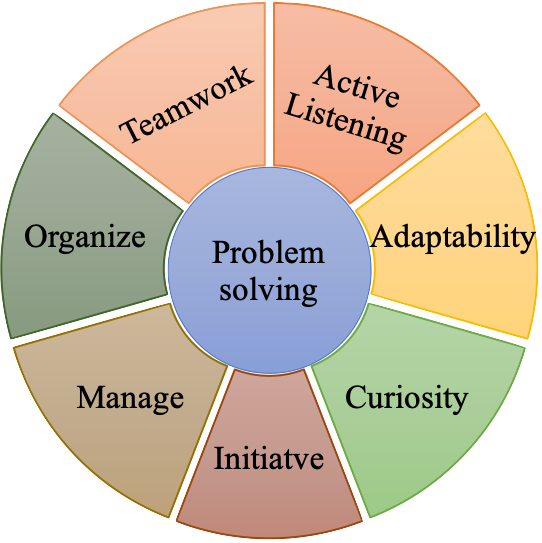
\includegraphics[scale=0.42]{img/personal.png}
~    
~
~
\section{Interests}
    \textbf{History}
    \textbf{Reading}
    \textbf{Photography}
    \textbf{Travel}
    \textbf{Hiking}
~    
~
~
  \section{Languages}
\textbf{English}
\includegraphics[scale=0.40]{img/5stars.png}
\textbf{Hindi}
\includegraphics[scale=0.40]{img/5stars.png}
\textbf{Bengali}
\includegraphics[scale=0.40]{img/5stars.png}
\textbf{Swedish}
\includegraphics[scale=0.40]{img/5stars.png}
~	
\end{aside}

\newpage
\section{Technical Skills}
\begin{entrylist}
\entry
	{Microbiology}
	{}
	{}
	{\begin{itemize}
	\item Liquid and solid cultures of bacteria and fungus (wood decay fungus, yeast), isolation, purification, transformation \item Isolation of two enzymes from wood decay fungi and further enzyme assay \item \textbf{Microscopy:} confocal, fluorescence and light microscopy \item Mix culture fermentation and distillation of alcohol \item Characterization of intracellular and extracellular microbial metabolites \item Wastewater treatment by white rod fungus \item Bio-surfactant production
	\end{itemize}}
	
\entry
	{Molecular Biology}
	{}
	{}
	{\begin{itemize} \item \textbf{Vector design:} primers design, digestions, ligations, cloning. \item \textbf{Cloning:} Genomic DNA isolation and purification, PCR, treatment with restriction enzymes, PCR product purification, ligations, transformation, DNA gel analysis, DNA sequencing. \item Cell-free enzymatic reaction
	\end{itemize}}
	
\entry
	{Biochemistry}
	{}
	{}
	{\begin{itemize} \item SDS PAGE \item Thin layer chromatography \item HPLC \item enzymatic assay
	\end{itemize}}
	
\entry
	{Polymer Chemistry}
	{}
	{}
	{\begin{itemize} \item \textbf{Polymer Characterization:} FTIR, XRD, SEM, AFM, tensile tester, GC-MS, HPLC, freeze dryer \item Surface tension measurements and handling of surfactant. \item \textbf{Separation:} Separation of lignin from black liquor and subsequent drying. Precipitation of bio-surfactant from bacterial culture by acid precipitation method. \item Natural and thermal aging of polyethylene with or without anionic surfactant. \item \textbf{Degradation:} Polyethylene and lignin. \item Starch polymer composite. \item Texttile dye adsorption.
	\end{itemize}}
	
\entry
	{Analytical Chemistry}
	{}
	{}
	{\begin{itemize} \item Titrations, spectrophotometry, chromatography (thin layer, ion exchange, HPLC), sound practical and theoretical knowledge and interpretations of most analysis techniques (NMR, MS, etc.).
	\end{itemize}}
\end{entrylist}

\section{Poster Presentation}
\begin{entrylist}
\entry
	{2014}
	{October 27th to 30th}
	{IIT Delhi, New Delhi, India}
	{International Conference on Polymeric Biomaterials, Bioengineering and Bio diagnostics}
	
\end{entrylist}

\begin{aside}
	~
	~
	~
	~
	\section{Professional community }
	\href{https://orcid.org/0000-0001-9754-9080}{
\includegraphics[scale=0.30]{img/orcid}}
	~
	\href{https://publons.com/researcher/2059651/shritama-mukherjee/}{
\includegraphics[scale=0.50]{img/publon}}
	~
	\href{https://www.researchgate.net/profile/Shritama_Mukherjee}{
\includegraphics[scale=0.60]{img/researchgate}}
	~
	\href{https://www.linkedin.com/in/shritama-mukherjee-93681267/}{
\includegraphics[scale=0.40]{img/linkedin}}
	~
	~
	~
	\section{Research Interests}
	Biomaterial synthesis
	Renewable polymer
	Environmental Microbiology
	Wate management
	Bioremediation
\end{aside}

\section{Conference attended}
\begin{entrylist}
\entry
	{2012}
	{Frontiers in modern biology (FIMB 2012)}
	{Indian Institute of Science Education and Research Kolkata, India }
	{}
\entry
	{2014}
	{International conference RAPT}
	{University of Calcutta, Kolkata}
	{}
\end{entrylist}

\newpage
\section{Referees}
\begin{entrylist}
	\entry
	{\textbf{Referee 1}}
	{Prof. P P Kundu, \\Professor\\Department of Chemical Engineering
		\\Indian Institute of Technology, Roorkee, India}
	{}
	{Email: \href{mailto: ppkfch@iitr.ac.in}{\textbf{PPKundu}@iitr.ac.in}\\
	\emph{Phone: +91 (0)725 1040 403}}
\\
\entry
	{\textbf{Referee 2}}
	{Prof. Uttam Raychoudhuri, \\Professor \\ Department of Chemical Technology, \\Calcutta University, West Bengal,India}
	{}
	{Email: \href{mailto: uttamraychaudhuri@yahoo.in}{\textbf{UttamRoyChaudhuri}@jyahoo.in}}\\
\entry
	{\textbf{Referee 3}}
	{Prof. Abhijit Bandyopadhyay, \\Professor \\ Department of Polymer Science \& Technology, \\Calcutta University, West Bengal,India}
	{}
	{Email: \href{mailto: abhijitbandyopadhyay@yahoo.co.in}{\textbf{AbhijitBandyopadhyay}@yahoo.co.in}}\\
	\end{entrylist}
\begin{aside}
~
	\end{aside}

%\begin{flushleft}
%\emph{March 31st, 2020}
%\end{flushleft}
%\begin{flushright}
%\emph{Jyotirmoy Das}
%\end{flushright}

\end{document}
